% !TeX spellcheck = <none>
%%
%% sample document for AAMAS'18 conference
%%
%% modified from sample-sigconf.tex
%%
%% see ACM instructions acmguide.pdf
%%
%% AAMAS-specific questions? n.yorke-smith@tudelft.nl
%%

\documentclass[sigconf]{aamas}  % do not change this line!

%% your usepackages here, for example:
\usepackage{booktabs}
\usepackage{graphicx}
\usepackage[rflt]{floatflt}
\usepackage{subcaption} 
\usepackage{frame, caption}
\usepackage{amsmath}
\usepackage{mathrsfs}
\usepackage{array}

\newcommand{\argmax}{\operatornamewithlimits{arg\,max}}

%% do not change the following lines
\setcopyright{ifaamas}  % do not change this line!
\acmDOI{doi}  % do not change this line!
\acmISBN{}  % do not change this line!
\acmConference[AAMAS'18]{Proc.\@ of the 17th International Conference on Autonomous Agents and Multiagent Systems (AAMAS 2018), M.~Dastani, G.~Sukthankar, E.~Andre, S.~Koenig (eds.)}{July 2018}{Stockholm, Sweden}  % do not change this line!
\acmYear{2018}  % do not change this line!
\copyrightyear{2018}  % do not change this line!
\acmPrice{}  % do not change this line!

%% the rest of your preamble here


%%%%%%%%%%%%%%%%%%%%%%%%%%%%%%%%%%%%%%%%%%%%%%%%%%%%%%%%%%%%%%%%%%%%%%%%%%%%%%%%%%%%%%%%%%%%%%%%%%%%%%%%%

%%%%%%%%%%%%%%%%%%%%%%%%%%%%%%%%%%%%%%%%%%%%%%%%%%%%%%%%%%%%%%%%%%%%%%%%%%%%%%%%%%%%%%%%%%%%%%%%%%%%%%%%%

\begin{document}
	
	\title{Guess the power of other: A computational model to reason about the interlocutor's behaviors in collaborative negotiation}  % put your title here!
	%\titlenote{Produces the permission block, and copyright information}
	
	% AAMAS: as appropriate, uncomment one subtitle line; check the CFP
	%\subtitle{Extended Abstract}
	%\subtitle{Industrial Applications Track}
	%\subtitle{Socially Interactive Agents Track}
	%\subtitle{Blue Sky Ideas Track}
	%\subtitle{Robotics Track}
	%\subtitle{JAAMAS Track}
	%\subtitle{Doctoral Mentoring Program}
	
	%\subtitlenote{The full version of the author's guide is available as \texttt{acmart.pdf} document}
	
	
	% AAMAS: submissions are anonymous for most tracks
	\author{Paper \#XXX}  % put your paper number here!
	
	%% example of author block for camera ready version of accepted papers: don't use for anonymous submissions
	%
	%\author{Ben Trovato}
	%\authornote{Dr.~Trovato insisted his name be first.}
	%\orcid{1234-5678-9012}
	%\affiliation{%
	%  \institution{Institute for Clarity in Documentation}
	%  \streetaddress{P.O. Box 1212}
	%  \city{Dublin} 
	%  \state{Ohio} 
	%  \postcode{43017-6221}
	%}
	%\email{trovato@corporation.com}
	%
	%\author{G.K.M. Tobin}
	%\authornote{The secretary disavows any knowledge of this author's actions.}
	%\affiliation{%
	%  \institution{Institute for Clarity in Documentation}
	%  \streetaddress{P.O. Box 1212}
	%  \city{Dublin} 
	%  \state{Ohio} 
	%  \postcode{43017-6221}
	%}
	%\email{webmaster@marysville-ohio.com}
	%
	%\author{Lars Th{\o}rv{\"a}ld}
	%\authornote{This author is the
	%  one who did all the really hard work.}
	%\affiliation{%
	%  \institution{The Th{\o}rv{\"a}ld Group}
	%  \streetaddress{1 Th{\o}rv{\"a}ld Circle}
	%  \city{Hekla} 
	%  \country{Iceland}}
	%\email{larst@affiliation.org}
	%
	%\author{Valerie B\'eranger}
	%\affiliation{%
	%  \institution{Inria Paris-Rocquencourt}
	%  \city{Rocquencourt}
	%  \country{France}
	%}
	%\author{Aparna Patel} 
	%\affiliation{%
	% \institution{Rajiv Gandhi University}
	% \streetaddress{Rono-Hills}
	% \city{Doimukh} 
	% \state{Arunachal Pradesh}
	% \country{India}}
	%\author{Huifen Chan}
	%\affiliation{%
	%  \institution{Tsinghua University}
	%  \streetaddress{30 Shuangqing Rd}
	%  \city{Haidian Qu} 
	%  \state{Beijing Shi}
	%  \country{China}
	%}
	%
	%\author{Charles Palmer}
	%\affiliation{%
	%  \institution{Palmer Research Laboratories}
	%  \streetaddress{8600 Datapoint Drive}
	%  \city{San Antonio}
	%  \state{Texas} 
	%  \postcode{78229}}
	%\email{cpalmer@prl.com}
	%
	%\author{John Smith}
	%\affiliation{\institution{The Th{\o}rv{\"a}ld Group}}
	%\email{jsmith@affiliation.org}
	%
	%\author{Julius P.~Kumquat}
	%\affiliation{\institution{The Kumquat Consortium}}
	%\email{jpkumquat@consortium.net}
	%
	%% The example's default list of authors is too long for headers
	%\renewcommand{\shortauthors}{B. Trovato et al.}
	
	
	\begin{abstract}  % put your abstract here!
		
		Interpersonal dominance relation has a major effect on the outcome of a negotiation. It has been shown that when participants adopt complementary dominance behaviors (one being dominant and the other being submissive), they reach mutually beneficial outcomes and this increases their reciprocal likings. In this paper, we investigate the simulation of this interpersonal relationship in the context of collaborative negotiation between an artificial agents.
		
		Our simulation is based on a previously published model. We present a Theory of Mind model that allows an agent to evaluate its interlocutor's level of dominance. The agent establishes the relation of dominance by adapting its behavior of power to complement the power of its interlocutor. We show on agent-agent simulation that the system correctly predicts the interlocutor's power. 
		
	\end{abstract}
	
	
	% AAMAS: the ACM CCS are not needed within AAMAS papers
	%%
	%% The code below should be generated by the tool at
	%% http://dl.acm.org/ccs.cfm
	%% Please copy and paste the code instead of the example below. 
	%%
	%\begin{CCSXML}
	%<ccs2012>
	% <concept>
	%  <concept_id>10010520.10010553.10010562</concept_id>
	%  <concept_desc>Computer systems organization~Embedded systems</concept_desc>
	%  <concept_significance>500</concept_significance>
	% </concept>
	% <concept>
	%  <concept_id>10010520.10010575.10010755</concept_id>
	%  <concept_desc>Computer systems organization~Redundancy</concept_desc>
	%  <concept_significance>300</concept_significance>
	% </concept>
	% <concept>
	%  <concept_id>10010520.10010553.10010554</concept_id>
	%  <concept_desc>Computer systems organization~Robotics</concept_desc>
	%  <concept_significance>100</concept_significance>
	% </concept>
	% <concept>
	%  <concept_id>10003033.10003083.10003095</concept_id>
	%  <concept_desc>Networks~Network reliability</concept_desc>
	%  <concept_significance>100</concept_significance>
	% </concept>
	%</ccs2012>  
	%\end{CCSXML}
	%
	%\ccsdesc[500]{Computer systems organization~Embedded systems}
	%\ccsdesc[300]{Computer systems organization~Redundancy}
	%\ccsdesc{Computer systems organization~Robotics}
	%\ccsdesc[100]{Networks~Network reliability}
	
	
	\keywords{Dominance; Reasoning about other; Theory of mind}  % put your semicolon-separated keywords here!
	
	\maketitle
	
	
	%%%%%%%%%%%%%%%%%%%%%%%%%%%%%%%%%%%%%%%%%%%%%%%%%%%%%%%%%%%%%%%%%%%%%%%%%%%%%%%%%%%%%%%%%%%%%%%%%%%%%%%%%
	%% start of main body of paper
	%
	
	\section{Introduction}
	Negotiation is a common task in daily life. People negotiate about simple situations as choosing a restaurant as well as complex situations such as salary negotiation or a promotion. Thus, we observe a variety of conversational agents which have been created to negotiate with people [refs]. Theses systems are designed with a large panel of abilities such as, the number of parties, the number of issues negotiated \emph{etc $\ldots$}.
	
	Negotiation is often complex to model. It is a multifaceted process which involves social interaction and affects as well as personal preferences and opinions  \cite{bro2010affective}. Indeed, researches in social psychology demonstrated that the relation of dominance affected the way that the negotiation precess is lived and perceived.
	Negotiating parties often differ in terms of power, and power differences exert an important influence on the way negotiator build their negotiation strategies, the behaviors displayed and by consequences the outcomes of the negotiation \cite{van2006power}. More precisely, dominance complementarity in which one negotiator exhibits high-power behaviors (dominant behavior) and other one responds with submissive behavior and vice versa \cite{tiedens2003power}. The complementarity leads the negotiator to reach mutually beneficial outcomes and increases their reciprocal likings \cite{wiltermuth2015benefits,tiedens2003power}.
	
	
	For our work, we aim to develop a system of collaborative negotiation that allows the agent to establish a complementary relation of dominance with the user. Thus, the agent adapts its behaviors to complement the behaviors of the user. 
	
	To construct a complementary relation of dominance, the agent has to interpret the user behaviors to understand the power he intends to express.  In a previous work \cite{ouali2017computational}, we designed a negotiation system capable of expressing negotiation's strategies that reflect the power of the agent. We propose to extend this model, with theory of mind abilities based on simulation, that allow the agent to reason about the behaviors. 
	
	Since the behaviors of power implemented reflects human behaviors, we assume that the user uses the same decision model. Therefore, the agent will define beliefs about the user' reasoning based on his  utterances. 
	
	
	In this paper specifically, we present our model of theory of mind that construct a mental model of the user and processes the value of power he exhibits in the negotiation. 
	
	The paper is organized as follow. Section II , provides background
	of previous automated negotiation agents with theory of mind and existing works on social behaviors recognitions. In section III, we present our model of dialogue of collaborative negotiation extended with theory of mind abilities. Section IV, presents our exepirements to validate our model. In section V, we present our conclusion and futur works.
	
	
	\section{Related works}
	
	In social interactions and negotiation in particular, reasoning about the beliefs, goals, and intentions of others is crucial. People use this so-called theory of mind \cite{premack1978does} or mentalizing to understand why others behave the way they do, as well as to predict the future behavior of others. Therefore, various negotiation models use Theory of Mind approaches to create models of negotiation which are more realistic. 
	
	For instance, Pynadath \textit{et al}\cite{pynadath2013you} showed the advantages of the theory of mind on negotiation even with an overly simplified model. They observed significant similarities between	the partner behavior and the agent's idealized expectations. Moreover, deviations in expectations about the other did not affect the agent performances and played in some cases in the advantage of the agent.
	
	de Weerd \textit{et al} \cite{de2013higher} investigated the use of high-order theory of mind in mixed-motive situations where cooperative and competitive behaviors play an important role. They found that the use of first-order and second-order theory of mind allow agents to balance competitive and cooperative	aspects of the game. This prevents the agents from breaking down compared to  agents without theory of mind.
	
	
	Theses presented works use dynamics which only focus on rational behaviors and exclude social aspects. However, The impact of social behaviors has been extensively debated in social psychology. Among such works, varios researches have been investigating emotion recognition in negotiation; the effects of one individual's	emotions on the other's social decisions and behavior during the negotiation. Moreover, they investigate how theses resource of information are integrated.
	For example, Elfenbein\textit{ et al} \cite{elfenbein2007reading} proved that  emotion recognition accuracy is positively correlated to  better performances in negotiation
	
	In the same vein, several researches suggested the effect of anger expression in the negotiation \cite{sinaceur2006get,van2010interpersonal,ferguson2004social}. For example, VanKleef \cite{van2004interpersonal} demonstrated that negotiators monitor their opponent's emotions and use them to estimate the opponent's limits, and modify their demands according to the presumed location of those limits. As a result, negotiators concede more to an angry opponent than to a happy one. 
	
	
	For theses reasons, reasoning about the social behaviors is important for the percpective of construnging negotiators agents. \cite{alfonso2015emotional} proposed a model that can observe and predict other's agents emotional behaviors. The three step method proposes to revise the agent's  beliefs by integrating a bayesian model which infers probabilities about the emotional behaviors of other's agents and compute probabilitistic prediction about their appraisals.
	
	Marcella \textit{et al} \cite{klatt2011negotiations} proposed a model of negotiation in the context of aid prevention. The model tries to combine handling of emotions with general structures of negotiations. 
	
	In the context our work, we focus on the impact of dominance in the negotiation. Dominance as an interpersonal relation is defined by burgoon \cite{burgoon1998nature} as expressive, relationally based communicative acts by which power is exerted and influence achieved. Futrthermore, its is a dyadic variable in which control attempts by one individual are accepted by the
	interactional partner \cite{dunbar2005perceptions}. For this reason, we focus on dominance complementarity between a negotiator agent and a human user in the context of collaborative negotiation. 
	
	Dominance complementarity is characterized by one person in adyadic interaction behaving dominantly and his counterpart behaving submissively \cite{tiedens2003power} have been investigated in the context of negotation. \cite{tiedens2003power} showed that when complementarity occurs in an interaction, people feel more comfortable and helps to create interpersonal liking relation.
	Moreover, \cite{wiltermuth2015benefits} showed that dominance complementarity can positively improve coordination and by consequences improve objective benefits.
	
	Our goal is to create a model of negotiation in which the agent adapts its negotiation strategies to the relation of dominance established with the user. Therefore, the agent has to reason about user's behaviors of power  to understand the level of dominance or submissiveness expressed. The agent then adopt a complementary starategy in order to complement the user behaviors and establish the relation of dominance.
	
	We present in this paper a model of theory of mind that build beliefs about the user behaviors of power in order to predict his behavior of dominance. We propose to use our model of negotiation based on power in order to reason about the user behaviors. 
	\section{Model of dialogue}
	
	We defined a dialogue system of cooperative negotiation which enable  a conversational agent to create and adapt its negotiation strategy to the power it intends to express. The goal of a negotiation is to choose an option from the discussed topic. Theses options are defined as a set of criteria  $\{C_1, ..., C_n\}$ that reflect the option's characteristics. In order to be able to negotiate about which option to choose, an agent is initiated with a set of partial or total ordered preferences $\prec_i$ defined for each criterion $C_i$. Using theses preferences, an agent can compute a score of satisfaction for each value of each criterion. The satisfaction of a value $v \in C_i$ is computed as the number of values that the agent prefers less in the preferences order $\prec_i$, then, the score is normalized in $[0, 1]$: 
	
	\begin{equation}
	sat(v, \prec_i) =	1 - \left( \frac{|\{v' : v' \neq v \  \wedge \ (v \prec_i v')\}| }{( |C_i| - 1 )}\right)
	\end{equation}
	
	The notion of satisfaction represents the score of liking for the value. The closer the satisfaction of a value $v$ gets to 1, the more the agent likes $v$. 
	
	\subsection{Model of decision based on power}
	The decisional process during the negotiation is built to take into account the power of the agent. Therefore, agent is initiated with a value of power $pow \in [0,1]$. In addition, the decisional process to produce an utterance considers respectively, the agent's power, its preferences and the context of the negotiation.  
	
	A detailed explanation of the decisional model is presented in \cite{} . We present in the following the most important factors that defines the agent strategy.
	
	\subsubsection{Satisfiability }
	\label{sec:sat}
	The agent is allowed to share its preferences. %(\emph{StatePreference(v)}). 
	To this end, the agent considers its perception of power $pow$ to compute the satisfiability, such that a value $v$ is satisfiable (likable), if:  
	\begin{equation}
	sat(v, \prec_i) \geq pow
	\end{equation}
	
	Therefore, given a value of $pow$, and a model of preferences $\prec$, the agent has a set of satisfiable values noted $S$. 
	
	\par For example, consider a mental state where $pow =0.6$, a criterion with a domain $D =\{A, B, C, D\}$ is defined with the set of preferences $ \prec_D = \{A \rightarrow  B, C \rightarrow  D , B \rightarrow D \}$. The values of satisfiability are depicted in the table \ref{sat}. We can compute that the set of satisfiable values is $ S = \{B, C, D\}$ 
	\begin{table}
		\centering
		\begin{tabular}{ |c|c|c|c|c| }
			\hline				
			value & A & B & C & D \\
			\hline
			
			\hline
			Sat(value) & 0.3 & 0.6 & 0.6 & 1 \\
			\hline
			
		\end{tabular}
		\caption{Value of satisfiability for the model $D$.}
		\label{sat}
	\end{table}
	
	
	\subsubsection{Acceptability}
	
	\begin{floatingfigure}[r]{1.5in}
		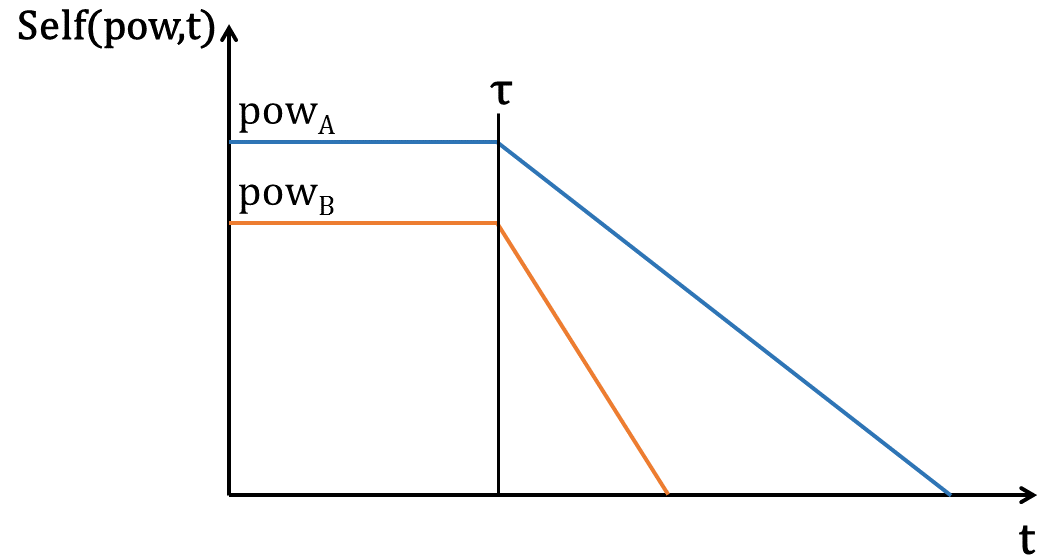
\includegraphics[width=1.5in]{figs/sv3.png}
		\caption{\label{fig:conc}Concession curve}
	\end{floatingfigure} 
	
	During the negotiation, the agent makes decisions about the proposals it receives. It might express an \emph{Accept} or \emph{Reject}. However, when the negotiation is not converging, the agent has to make concessions which means that the agent has to lower his level of demand. 
	We compute the notion of concession with $self(t)$, which is a time varying value of $pow$ that decreases over time $t$. In the beginning, $self(0) = pow$, when the negotiation evolves without converging self decreases $self(t) < pow$ as presented in the figure \ref{fig:conc}.
	
	
	Thus, a proposal with a value $v \in C_i$ is \emph{acceptable} ($v \in Ac$) is computed with a boolean function:
	\begin{equation}
	acc(pow, v) = sat(v, \prec_i) \geq self(t)
	\end{equation}	
	and we note $Ac$ the set of acceptable values.
	
	%When negotiation progress in time without converging to a trade-off,
	In addition, When concessions occurs during the negotiation $self(t) < pow$. As a consequence, the agent might accept proposals which are not satisfiables. We note $M$ the set of acceptable values which are not satisfiables.
	$\{v \in M / v \in Ac, v \notin S\}$.
	
	%	Therefore, in order to accept \emph{Accept} or propose \emph{Propose} a value $v$, this value has to be acceptable $v \in Acc$. In the contrary, a value $v$ can be rejected (\emph{Reject}) if $v \not \in Acc$ and by consequences $v\not \in S$
	%	
	\subsubsection{Lead of the dialogue}
	The agent uses a strategy to choose the utterance type that reflects behaviors of power. Indeed, high-power agents focus on utterances of \emph{propose} in order to make the negotiation go on. On the contrary, a low-power agent uses in average more \emph{ask} utterances in order to have an accurate knowledge about the other to take the fairest decision.
	
	\subsection{Beliefs about other}
	
	In order to build a complementary relation of dominance with the user, the agent has to construct beliefs about the behaviors of power expressed by the user and adapt to complement his behavior. 
	
	We make the assumption that our model of dialogue effectively presents the process of utterance's selection using power. 
	
	Based on this assumption, we propose to enable the agent with a model of theory of mind based on simulation \cite{bibid}. The agent uses its model of decision in order to guess the behavior of the user from its enunciated utterance.   
	
	The agent needs to infer hypotheses about the user's mental state (\emph{i.e} Pow, Preferences) in order to reason about his behaviors. With knowledge gathered during the negotiation, the agent will remove inconsistent hypotheses.
	
	First, we define hypotheses about the possible values of $pow$ that the agents aims to predict. Let $H_{pow} = \{0.1, 0.2, \ldots, 0.9\}$ be the hypotheses on $pow$.
	
	Second, for each fixed hypothesis $ h_i \in H_{pow}$, we define hypotheses on the different set of preferences  noted $M_H $. Thus, for each criterion $C_i$ of the a topic , we compute all the possible combination of preference's relations. When relations of preferences are total ordered, the total number of preference's relations is in the order of $|H{C_i}| = |C_i|!$. In the case of partial ordered relations of preferences, the total number of possible relations is  $ |H{C_i}| = (|C_i| + 1)!$. Hence, for a topic of negotiation with $n$ criteria, the number of possible set of preferences is 
	$$ |M_H| = \prod_{i=1}^n (|H{C_i}|)$$ .
	
	For each hypothesis $ h_i \in H_{pow}$, we associate the set of possible preferences $M_H(h_i)$ identical for all the hypotheses in the beginning. After each user's turn, the agent updates its hypotheses and remove the ones that did not produced the same utterance than enunciated by the user. The value of power selected is computed as follow:
	
	\begin{equation}
	pow_{Other} = \operatorname*{arg\,max}_{h_i \in H_{pow}} (M_H(h_i))
	\end{equation} 
	
	This solution presents a computational limitation concerning the number of hypotheses formulated to generate the preferences. As presented, the size of hypotheses $M_H$ is considerable which can slow down the dialogue generation. However, we don't aim to know the "correct" preferences of the user but only the expressed power $pow$. 
	
	To deal with this limitation, we propose to infer hypotheses with partial knowledge about preferences. We only need to represent information about the user's preferences to be able reproduce its decisional model. 
	
	
	
	\subsection{Partial model of preferences}
	
	The model of preferences is used to compute the satisfiability of values (see section \ref{sec:sat}). Knowing the set of satisfiable values is crucial for the decisional process. Therefore, instead of computing hypotheses on the set of preferences, we propose to compute hypotheses about $S$, the set of satisfiable values for a giving value of power $pow$.  
	
	\par In order to generate theses hypotheses for any criterion, we make the strong assumption that preferences are \emph{total ordered.} In this case, all the values are comparable and could be ranked by order of preferences. Knowing the rank of preferences allows the agent to compute in advance the possible values of satisfiability.
	
	For example, the criterion $D$, of the size  $|D| = 4$ with total ordered preferences, get the values of satisfiability as presented in table \ref{tab:poss}.
	\begin{table}[h]
		\centering
		\begin{tabular}{ |c|c|c|c|c| }
			\hline				
			rank(value) & 1 & 2 & 3 & 4 \\
			\hline
			Nb predecessors & 3 & 2 & 1& 0 \\
			\hline
			Sat(value) & 0 & 0.33 & 0.66 &1 \\
			\hline
			
		\end{tabular}
		\caption{Values of satisfiability for the criterion $D$.}
		\label{tab:poss}
	\end{table}
	
	Based on the values of satisfiability, and given a fixed value of $h_i \in H_{pow}$, we can compute the size of $S$ in order to generate hypotheses on the different combination of satisfiable values  noted $M_h(h_i)$. For example, considering a value of $pow =0.6$, and the same criterion $D$, the number of satisfiable values $|S| = 2$. Therefore, $M_h(pow) = \{(A,B), (A,C), (A,D), (B,C), (B,D), (C,D)\}$. This process is generalized to all the hypotheses of $H_{pow}$. An example is presented in the table \ref{sat}
	
	
	
	
	\begin{table}[h]
		\centering
		\begin{tabular}{ |c|c|c| }
			\hline
			& \multicolumn{2}{c|}{Hypotheses}  \\
			\hline
			Hypothesis & pow & $M_h(pow)$ \\
			\hline
			H1&0.3&$\{ (A,B,C) , (A,B,D), (A,C,D), (B,C,D) \}$ \\
			\hline
			H2&0.4&$\{ (A,B), (A,C), (A,D), (B,C), (B,D), (C,D) \}$ \\
			\hline
			H3&0.5&$\{ (A,B), (A,C), (A,D), (B,C), (B,D), (C,D) \}$\\
			\hline
			H4&0.6&$\{ (A,B), (A,C), (A,D), (B,C), (B,D), (C,D) \}$ \\
			\hline
			H5&0.7&$\{ (A), (B), (C), (D) \}$\\
			\hline
			H6&0.8&$\{ (A), (B), (C), (D) \}$ \\
			\hline
			H7&0.9&$\{ (A), (B), (C), (D) \}$ \\
			\hline
		\end{tabular}
		\caption{Hypotheses on mental states for the criterion $D=\{A, B, C, D\}$}
		\label{table:poss}
	\end{table}
	
	\subsection{Decision in negotiation with partial representation of preferences}
	The adaptation of the mental state to partial representation implies to modify the reasoning process. In the following, we present the adaptation of the decisional model to take into account partial and incomplete mental state. The goal is to reproduce the reasoning model in order to compute at each turn, the power $other_{pow}$ of the interlocutor. 
	
	First, we present the adaptation of the functionalities. Second, we present, the computation of the other's \emph{pow} from functions of decision.   
	
	\subsubsection{Satisfiability:}
	To compute whether a value $v \in C_i$ is satisfiable, we check for each hypothesis of power $h_i$, the set satisfiable values $S_i \in M_h(pow)$.
	Thus: 
	\begin{equation}
	sat_{S_i}(v)= \left\{\begin{array}{ll}
	True	 & \mathrm{if\ }  v \in S_i\\
	False & \mathrm{otherwise}
	\end{array}\right.
	\end{equation}
	
	\subsubsection{Acceptability:}
	Computing the acceptability of a value $v$ depends on the current of value of $self(t)$. For each hypothesis on power $h_i$, we associate a value $self_i(t)$ that represents the level of concessions at the current time. 
	
	With partial knowledge of preferences and for a fixed value of power $h_i$, the agent is not able to compute all the acceptable values $Ac_i$. Especially,   values of the set $M_i$ (\emph{i.e} acceptable values which are not satisfiable). 
	
	Nevertheless, the agent can have certain information about acceptable values such as $ S_i \subset Ac_i$. Moreover, using the initial values of satisfiability for a given criterion (see table \ref{sat}), agent can compute the number of acceptable values at the current state of the negotiation $|Acc_i|$ and by consequences $|M| = |Acc_i| - |S_i|$. 
	
	We propose to calculate the score of acceptability of a value $v$ taking into account the available information. Therefore, for a hypothesis of power $h_i$, hypotheses on preferences $S_i \in M_h(h_i)$,  and the list of accepted values during the negotiation $A$, the score that $v \in D$ is acceptable is computed as follow: 
	\begin{equation}
	Acc(v, pow) = C_{|D|-(|S_i| + k)}^{|M| - k}
	\end{equation}
	$k = |K| $ is the number of elements in the set $K = A \cap \overline S_i$
	
	
	
	\subsection{Update hypotheses about pow}
	At each turn of the dialogue, the agent uses its model of the theory of mind in order to compute other's behaviors of power $pow_{other}$. We present, the process of updating $other_{pow}$ depending on the received utterance. 
	\subsection{Lead of the dialogue}		
	As presented before, the choice of a specific utterance's type translates behaviors of power. Indeed, a high frequency of choosing \emph{proposal utterance} shows a behaviors of high-power. Whereas, a high frequency of \emph{share preferences utterances} reflects behaviors of low-power.
	We note $history$ the list of utterances enunciated by the user. the value of power is computed from the ratio of propose enunciated versus asks.
	\begin{equation}
	pow_{other} = \left\{\begin{array}{ll}
	> 0.5 & \mathrm{if } \frac{history(Propose)}{hisotry} > 0.5\\
	\leq 0.5 & \mathrm{if  } \frac{history(Ask)}{hisotry} > 0.5
	\end{array}\right.
	\end{equation}
	
	Once, the list of possible is restricted, we update the hypotheses by taking into account the value associated to the expressed utterance.
	
	\subsubsection{Share a preference}
	When the user expresses a \emph{StatePreference(v, s)}, he shares his preferences in the way where $v \in S$ if $s =true$, otherwise $v \notin S$. 
	In addition, when the user rejects a proposal \emph{Reject(p)}, he also shares his preferences . As $S \subset Acc$ means if a value is not acceptable, it is automatically not satisfiable $p \notin S$. 
	
	Therefore, for each  $h_i \in H_{pow}$, we propose to update the agent's hypotheses $M_h(h_i)$ by removing all the hypotheses on preferences that are no longer consistent with the information learned. 
	Then, we compute the score of each $h_i$ at the moment $t$ :
	
	$$score(h_i,t) = \frac{|M_h(h_i, t)|}{|M_h(h_i, init)|}$$
	
	The value of power selected:
	\begin{equation}
	pow_{other} = \operatorname*{arg\,max}_{h_i \in H_{pow}} ( score(h_i,t))
	\end{equation}
	
	\subsection{Accept a proposal}
	When the user accept (\emph{Accept(p)}) or propose a proposal (\emph{Propose(p)}), means that $p \in Acc$. 
	The agent has to calculate for each $h_i \in H_{pow}$ the score of acceptability. In addition, the values of acceptability have to be normalized to allow a coherent comparison. Thus, given a hypothesis on power $h_i$, he score of acceptability is normalized by taking into account the ideal score of acceptability.
	
	$$I_{pow} =  C_{|D|-|S_i|}^{|M|}$$
	
	
	The final value of acceptability is then:
	\begin{equation}
	score(h_i, t)= \left( \begin{array}{c}  \frac{1}{I_{pow}} \cdot \sum_{S_i \in M_h(h_i) } acc(p, h_i) 
	\end{array}\right) \frac{1}{| M_h(h_i)|}
	\end{equation}
	
	Finally, the value of power is selected using the function (7) presented earlier.
	
	
	\section{Evaluation}
	In this section, we present our simulation study to show the acceptability of our model of dialogue. We aim to evaluate the accuracy of our model of theory of mind as well as the timeliness of the algorithm.
	
	\subsection{Method}
	
	We imeplemented two agents with thoery of mind abilities.
	The first agent ($agent_A$) plays a role of a dominant agent( $pow > 0.5$), whereas, the second agent ($agent_B$) plays the role of a submissive agent ($pow \leq 0.5$). 
	We manipulated two simulation parameters for the initialisation of our agents. First, the power of both agents (named \emph{pow-a} and \emph{pow-b}). We variate the values of power in order to study the accuracy in different settings as presented in table \ref{tab:powsettings}.
	Second, we variate the preference sets and more specificly the size of the discussed topic in order to study the timeliness of the algorithme from simple to richer topics. We generate $150$ different models of preferences.
	
	In total we generate $1451$ combinations for the initial states of both agents. For each combination, we generate a dialogue in which the agent with theory of mind estimates the other's value of power.
	
	\begin{table}[t]
		\centering
		\begin{tabular}{|l|cccc|}
			\hline 
			\textbf{Dominance value } &	\multicolumn{4}{c|}{ Initial values of power } \\
			\hline
			Dominant agent $pow_A$ & 0.3 & 0.4 & 0.5 &  \\
			\hline
			Submissive agent $pow_B$ & 0.6 & 0.7 & 0.8 & 0.9\\
			\hline
		\end{tabular}
		\caption{Initial condition's setting for the values of power} 
		\label{tab:powsettings}
	\end{table}
	
	\subsection{Results and discussion}
	We present in this section the results obtained for both the accuracy of model and the timeliness of the execution.
	
	\subsubsection{Accuracy of predictions:} For each dialogue, we obtain the prediction of power of one agent, and the results are depicted in table \ref{tab:res1}. 
	First, we computed the standard deviation between the actual value of powe $pow$ and the guessed value of power $Other_{pow}$. In average, for the total $1451$ dialogues, a small deviation of was observed. Moreover, in order to analyse the results in a more general way, we calculated the \emph{risidual deviation } in order to compute the deviation of the observed value of power $Other_{pow}$ from the
	real value of power $pow$. 
	We observe small deviations which means that our model makes close predictions of behaviors  related to power of the other agent.
	\begin{table}[h]
		\centering
		\begin{tabular}{|l|c|}
			\hline
			Average of the standard deviation & 0,075 \\
			\hline
			Risidual variation & 0,015 \\
			\hline
		\end{tabular}
		\caption{Results of margin errors for prediction} 
		\label{tab:res1}
	\end{table}
	
	Second, we analyzed the frequency of false predictions. For example, $agent_A$ predicts that $agent_B$ is dominant whereas $agent_B$ is submissive. Therefore, we computed percentage of false prediction which at the order of $ 2.6 \% $. Indeed, only $30$ predictions were incorrect. This result enhance the reliability of our algorithm. 
	
	Finally, we studied the stability of our algorithm. For each dialogue, we computed the number of iterations necessary to find the best $Other_{pow}$. The results depicted in graphs show the residual variation at each iteration for the different topics. We observe that in average, after $7$th itertation, the algorithm converges to a final value of $other_{pow}$.
		\begin{table*}[t]
		\begin{tabular}{|c|c|c|c|c|c|c|c|c|c|}
			\hline
			\textbf{$Other_{pow}$} & \multicolumn{9}{c|}{Number of iteration } \\
			\hline
			Small &0,047&0,071&0,063&0,016&0,010&0,009&0,011&0,011&0,011 \\
			\hline
			Medium&0,058&0,084&0,075&0,030&0,017&0,016&0,017&0,017&0,017\\
			\hline
			Large&0,052&0,116&0,099&0,024&0,015&0,015&0,017&0,017&0,018 \\
			\hline
			
		\end{tabular}
		\caption{Results of margin errors for prediction} 
		\label{tab:conv}
	\end{table*}
	
	Moreover, we studied the impact of the number of hypotheses on the stability. We wanted to study wether a large number of hypotheses will need extra iterations to converge. Therefore we compared results obtained for small topic, medium, and large topics of conversation. The graph presented in figure \ref{converge} shows that our algorithm converges in average quickly independtly from the size of topic. The data presented in table \ref{tab:conv}, we observe that the algorthim took two additional iterations to converge in the large topic. The difference is not significant.
	
	
		\begin{figure}[]
			\fbox{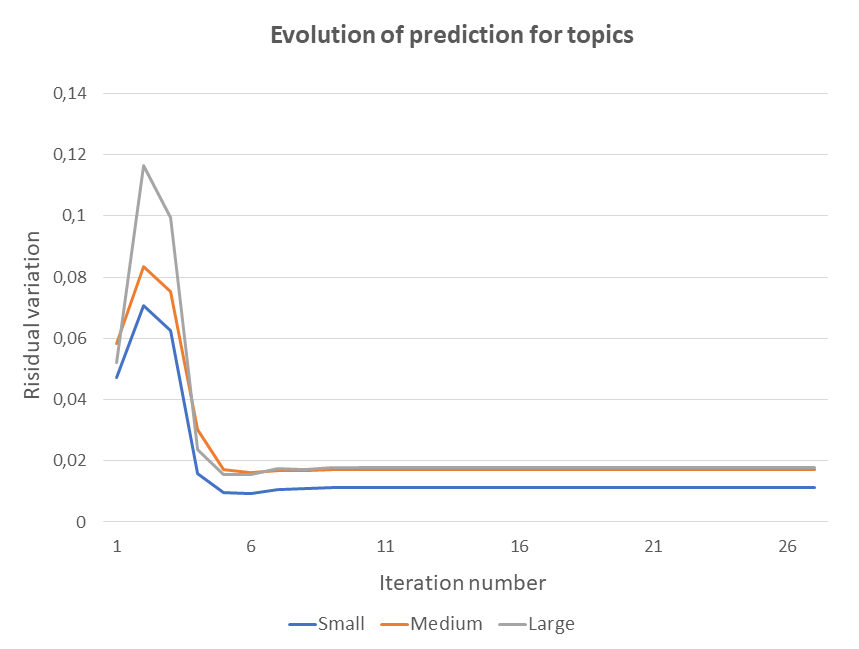
\includegraphics[width=\linewidth]{figs/total.PNG}}
			\caption{Algorithm convergence for all topics} 
			\label{converge}
		\end{figure}
	
	
	\subsection{Timeleness}
	We evaluate the time excution of the algorithm in order to study how the model of theory of mind evolves.For each dialogue, we computed the time excution of the negotiation. Results are presented in figure \ref{fig:time}, where wee see the evolution of the time execution. Unfortunatly, the evolution of the algorithm is exponential.
	\begin{figure}
		\fbox{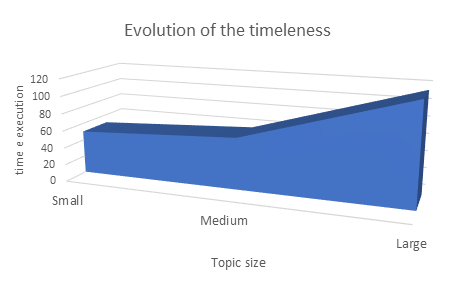
\includegraphics[width=\linewidth]{figs/time.png}}
		\caption{Time execution for the different topics}\label{fig:time}
	\end{figure}
%	\begin{figure*}[t]
%		\minipage{0.3\textwidth}
%		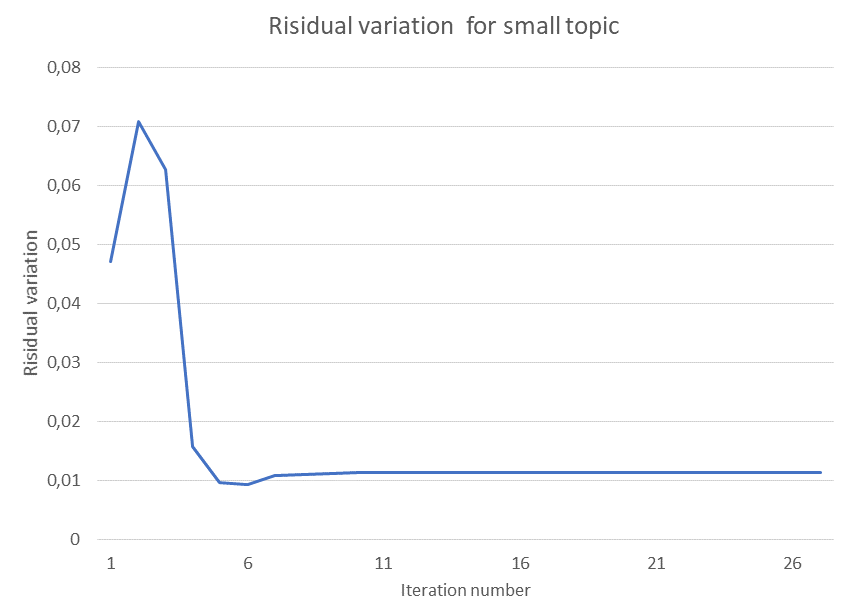
\includegraphics[width=\linewidth]{figs/small.png}
%		\caption{A really Awesome Image}\label{fig:small}
%		\endminipage\hfill
%		\minipage{0.3\textwidth}
%		\fbox{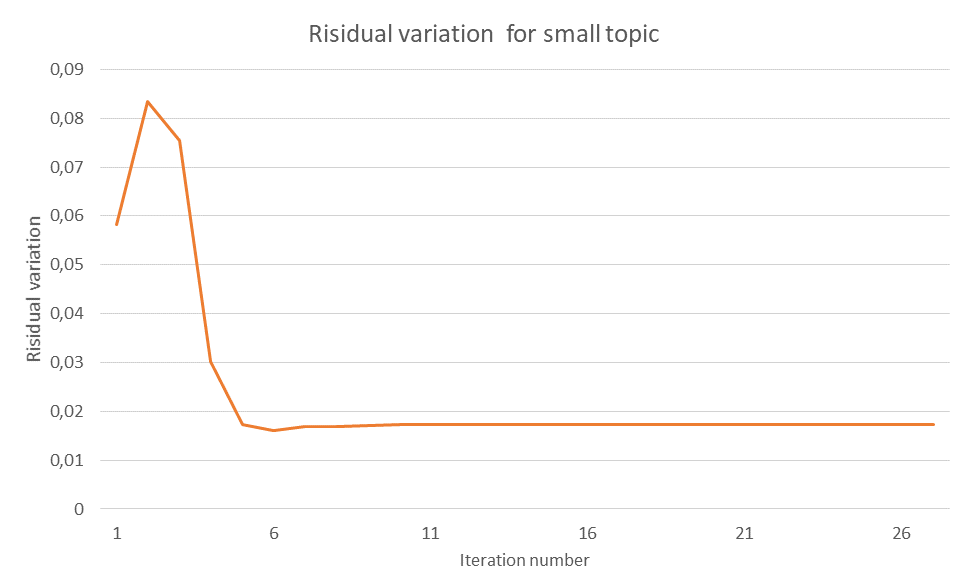
\includegraphics[width=\linewidth]{figs/medium.png}}
%		\caption{A really Awesome Image}\label{fig:medium}
%		\endminipage\hfill
%		\minipage{0.3\textwidth}%
%		\fbox{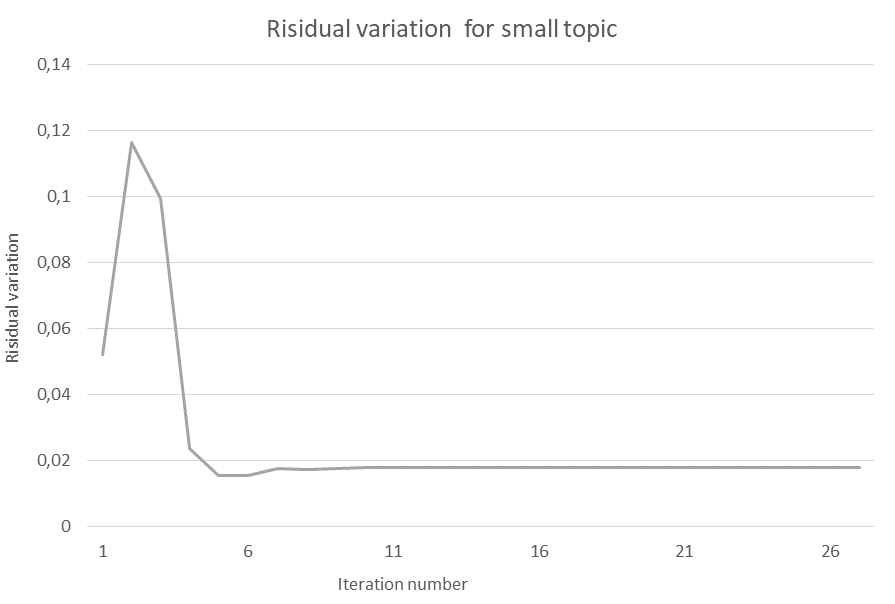
\includegraphics[width=\linewidth]{figs/large.png}}
%		\caption{A really Awesome Image}\label{fig:large}
%		\endminipage
%	\end{figure*}
%	
	\section{Discussion}
	\section{Conclusion}
	%%%%%%%%%%%%%%%%%%%%%%%%%%%%%%%%%%%%%%%%%%%%%%%%%%%%%%%%%%%%%%%%%%%%%%%%%%%%%%%%%%%%%%%%%%%%%%%%%%%%%%%%%
	%% bibliography: see CFP for number of permitted pages
	
	\bibliographystyle{ACM-Reference-Format}  % do not change this line!
	\bibliography{bibliography}  % put name of your .bib file here
	
\end{document}